\chapter{Models and Associated Probes For Proton Spin Structure}
\begin{figure}
  \centering
  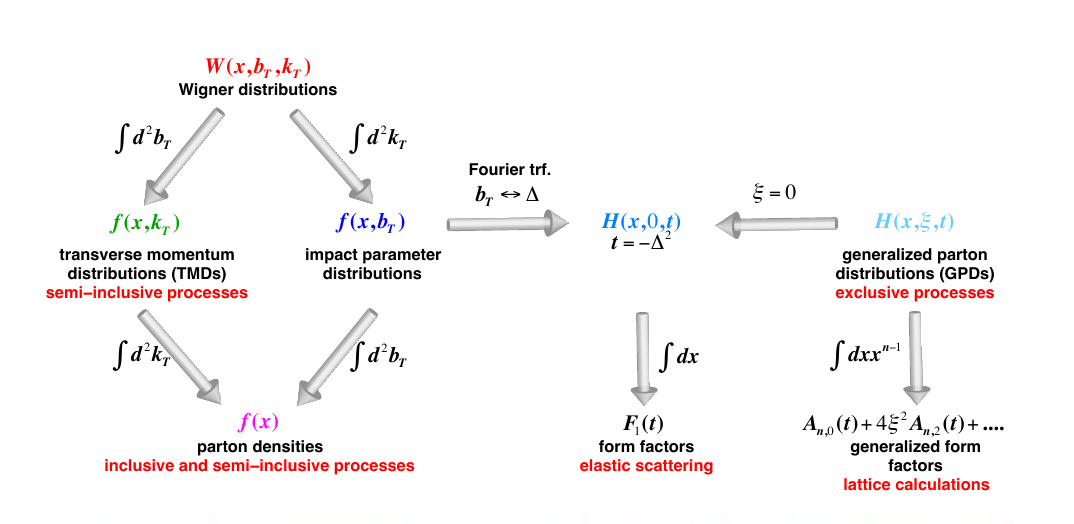
\includegraphics[width=\linewidth]{./figures/pdf_distributions_invariants.png}
  \caption{
    Figure from \cite{Accardi2012}.
  }
  \label{fig:invariants_observables_pdf}

\end{figure}
\section{ Structure Functions}
Spin structure overall: \cite{Accardi2012} pp 29-31
Longitudinal spin structure: \cite{Accardi2012} pp 32-43

\begin{figure}
  \centering
  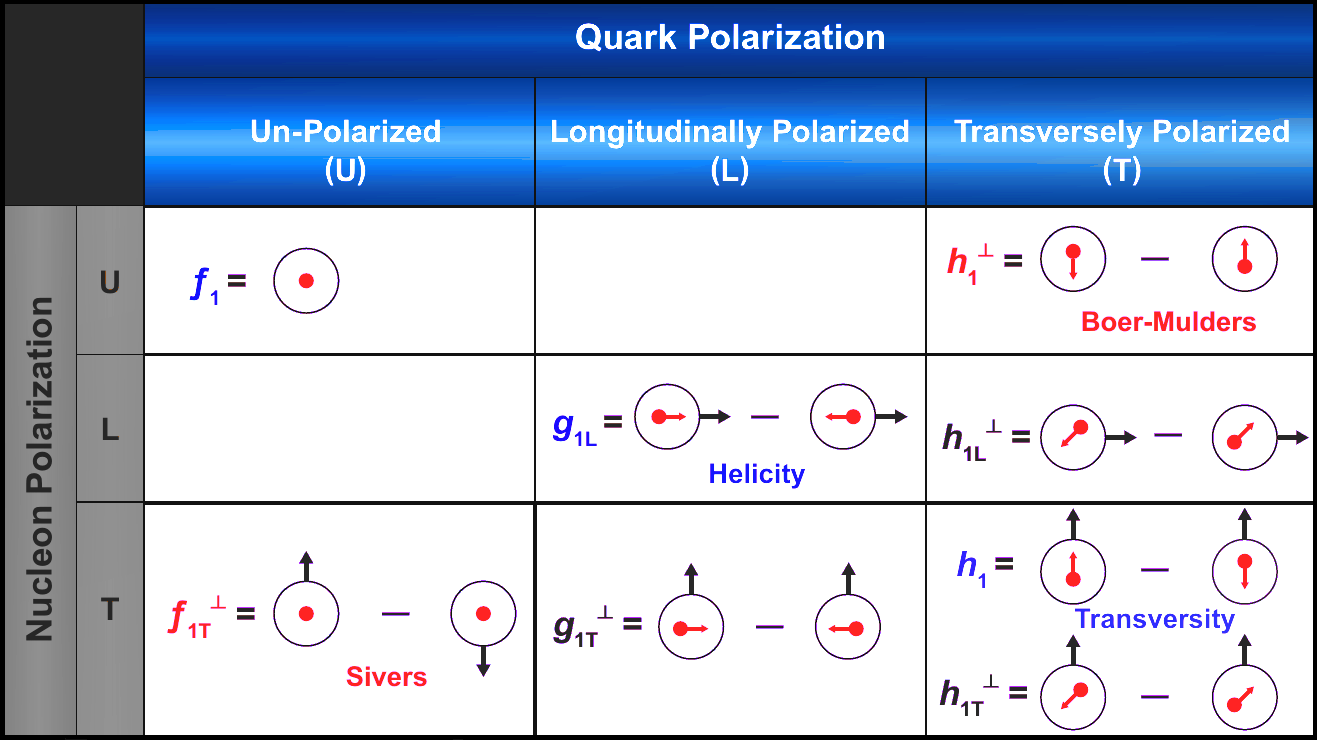
\includegraphics[width=\linewidth]{./figures/leading_twist_polarization_config.png}
  \caption{
    Figure from \cite{Accardi2012}.
  }
  \label{fig:leadings_twist_probes}
\end{figure}

\section{ proton spin decomposition}
\section{ unpolarized parton distribution functions}
\section{ polarized parton distribution functions}
\section{ that sweet table from Delia hasch}
\section{ discussion $\bar{q}$, $q$, $L_q$, $g$}
\section{ DSSV }

\clearpage
\section{Measurement of the Proton Spin}
\subsection{ physics probes for proton spin}
\subsection{ W cross section}
\subsection{ derivation of Asymmetry}
\subsection{ kinematic extremes of Asymmetry}

\clearpage
\section{Cross Sections and Luminosity}
\begin{itemize}
		\item vernier analysis note intro, equations
		\item summarize the papers on Lumoninosity
\end{itemize}

\clearpage
